\documentclass{article}
\usepackage{blindtext}
\usepackage{geometry}
\usepackage{graphicx}
\usepackage{ragged2e}
\usepackage{hyperref}
\graphicspath{ {./images/} }
 \geometry{
 a4paper,
 total={170mm,257mm},
 left=20mm,
 top=20mm,
 }
\usepackage{multicol}
\title{\textbf{Mass Spring Model with BVH Cutting Cloth Technique}}
\author{Siravich Sereepong, \\ 
Digital Design \& Creative Technology, \\
King Mongkut's University of Technology Thonburi}
\date{June 2024}
\begin{document}
\maketitle

\begin{multicols}{2}
\section*{Abstract}
\textbf{\indent This approach of the cloth simulation's behavior was based on various research papers and combined those methods into this paper. This will focus on both graphics rendering techniques and applied physics which are spring formula and Euler method to enhance results in terms of realistic.}

\textbf{\indent This paper will walkthrough how we can illustrate the cloth in the scene as well as how to handle both simple collision and raycasting which will represent as a mouse event. The sample of the project will be provided as a custom engine created by the OpenGL graphics library with C++.}

\section{Introduction}
\indent \indent Cloth is a material which contains millions of packed threads which we cannot simulate that amount of objects in the scene. By the way, there are some techniques in which we can render those cloth into the scene called ``Mass Spring Point''. The mass spring point will sample points in the cloth that have their own mass and will be applied by the spring force of neighboring points.
In terms of physics, we can calculate the spring force by using Hooke's Law along with Newton's Law which will extract force into the acceleration. After calculating those values, it will be used to compute the change of position by using Euler's method, differential of acceleration and velocity, to get the change of position in specific change of time.

\indent After dealing with physics, we can use those data to visualize the scene and by visualizing we have to prepare the buffer as well as the vertex data including position, normal and the output texture. This project used deferred shading technique which is easy to understand and debugging. The challenging point in this project is how we will illustrate the interaction between the user and the cloth itself. To clarify, the program must handle the mouse events for dragging and cutting the cloth which led to the introduction of the Bounding Volume Hierarchy(BVH). It plays a big role on how we can optimize this program.

\columnbreak
\section{Implementation}
\subsection{Physics}
First of all, before computing the physics of the mass spring point. We have to illustrate what the cloth will look like.

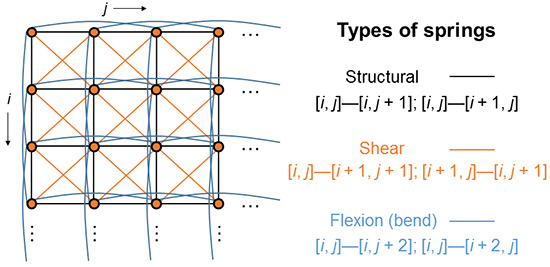
\includegraphics[width=\linewidth]{MassSpringPoint}
\centering [Figure 2.1.1 : Types of springs]\newline

\justifying
As we can see from 2.1.1, the type of spring we will use is the force between their consecutive directions including slant and bending which are 12 directions. Then applying various force which are spring, gravitational, damping force.\newline

\raggedright Hooke's Law:\\
\centering $F = k\Delta x$\\
\raggedright Gravitational Force:\\
\centering $F = mg$\\
\raggedright Newton's Law:\\
\centering 
$\Sigma F = ma$\\
$k\Delta x + mg = ma$\\
$a = \frac{(k\Delta x + mg)}{m}$

\raggedright
Note:\\
$k$ = Spring Constant\\
$\Delta$x = Length between point\\
$m$ = Mass of point\\
$g$ = Gravity Constant\\
$a$ = Acceleration\newline

\justifying
After we plugged all of variables, we will get a acceleration ``a'' and will perform Euler's method as well as differential both acceleration and velocity respectively.\newline

\raggedright Euler's Method:\\
\centering $v_{t} = v_{t-\Delta t} + a \times \Delta t$\\
\centering $x_{t} = x_{t-\Delta t} + v \times \Delta t$\\

\justifying
\indent We will keep values of both $x_t$ and $v_t$ for computing in the next frame. On the other hand, we can discard the acceleration after computing Euler's method since the acceleration that we get will change in every frame.
Also, the value of $\Delta t$ can be represented as a difference of time in each frame and since each machine has different hardware so the output as well as the frame rate of the output will be different also. To fix that, we can define the fixed time step value to lock the $\Delta t$ in each frame so that each frame will run at the same speed and we can tune the time step value by ourselves also to make it simulation fast or slow.
Making the time step too large or slow will cause distorted output because the simulation was too fast or slow and the cloth cannot finish computing in that time.
\subsection{Rendering}
In the rendering part, this paper will seperate into 2 parts which are deferred shading, cloth interaction.
\subsubsection{Deferred Shading}
Deferred shading technique is quite widely in the graphics field which can be seperate the image buffers into 4 parts including position, normal, diffuse/albedo and depth buffers. Each of them have their own unique data that will use in lighting calculation. By combining all of buffers, we will get a complete data for calculating the light. 
Deferred shading is easy to implement and faster than forward shading when our scene contains lots of light sources.\newline

\centering
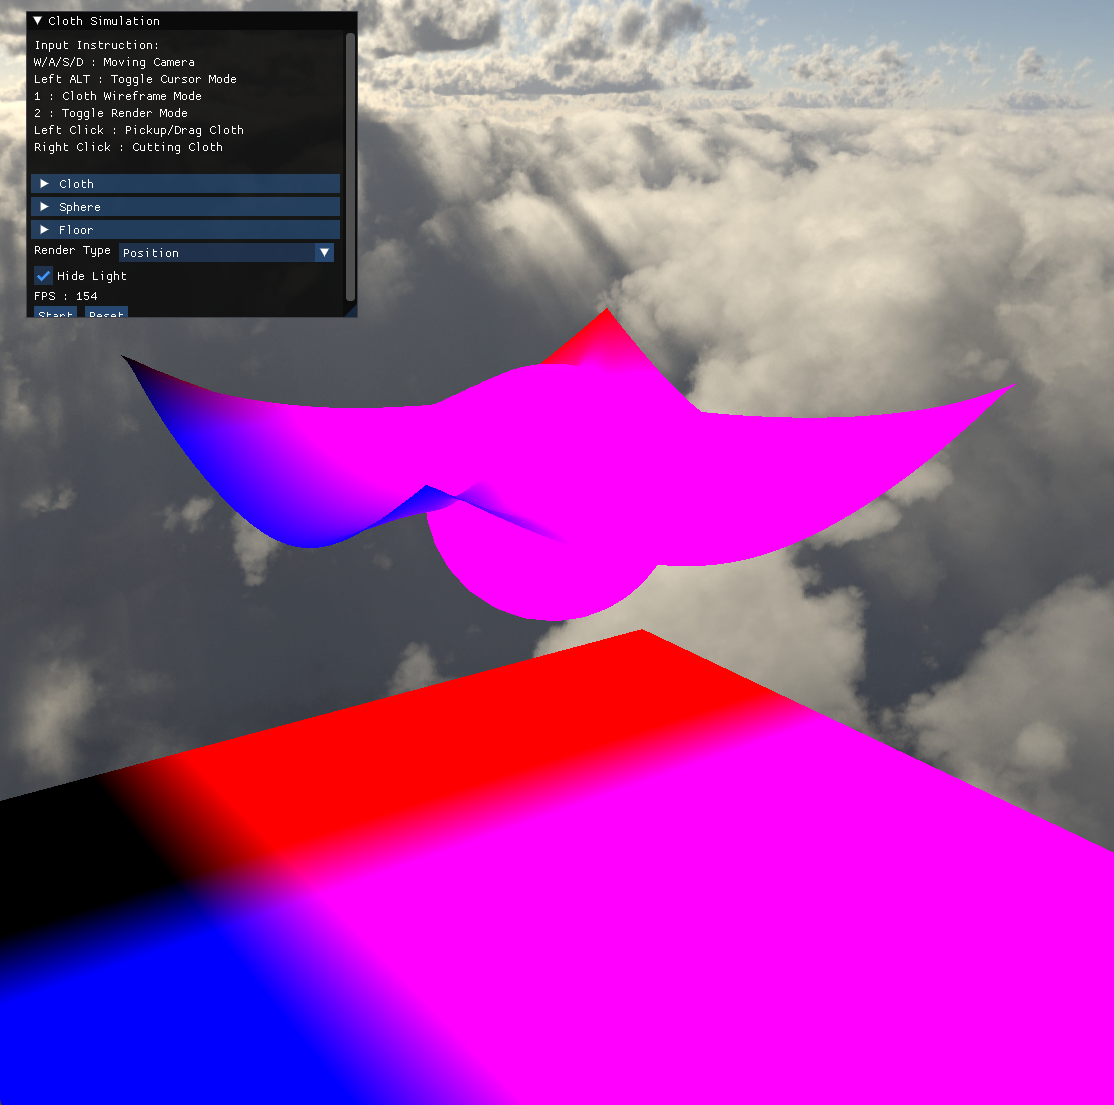
\includegraphics[scale = 0.2]{Deferred_Position}
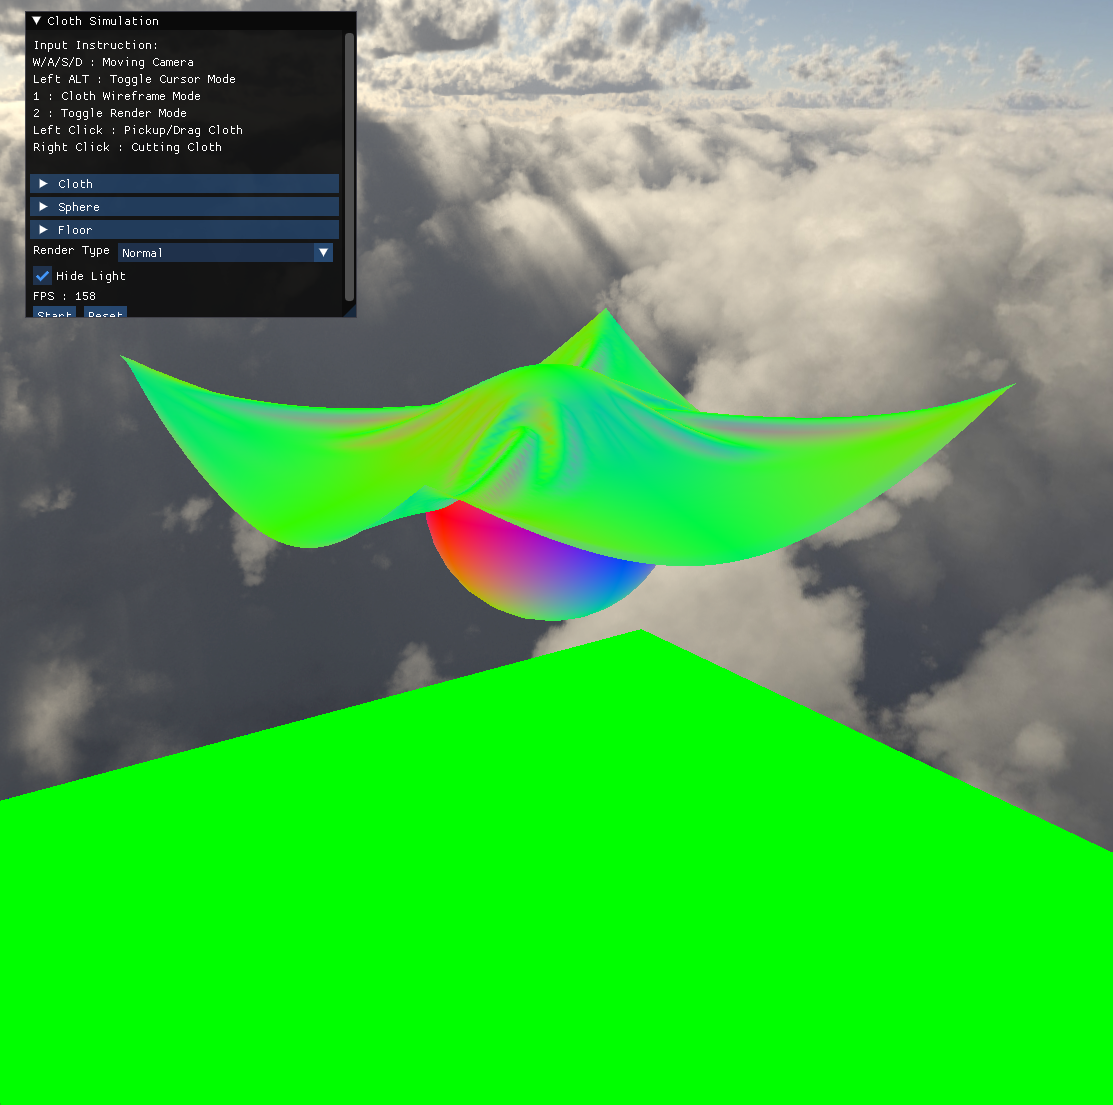
\includegraphics[scale = 0.2]{Deferred_Normal}
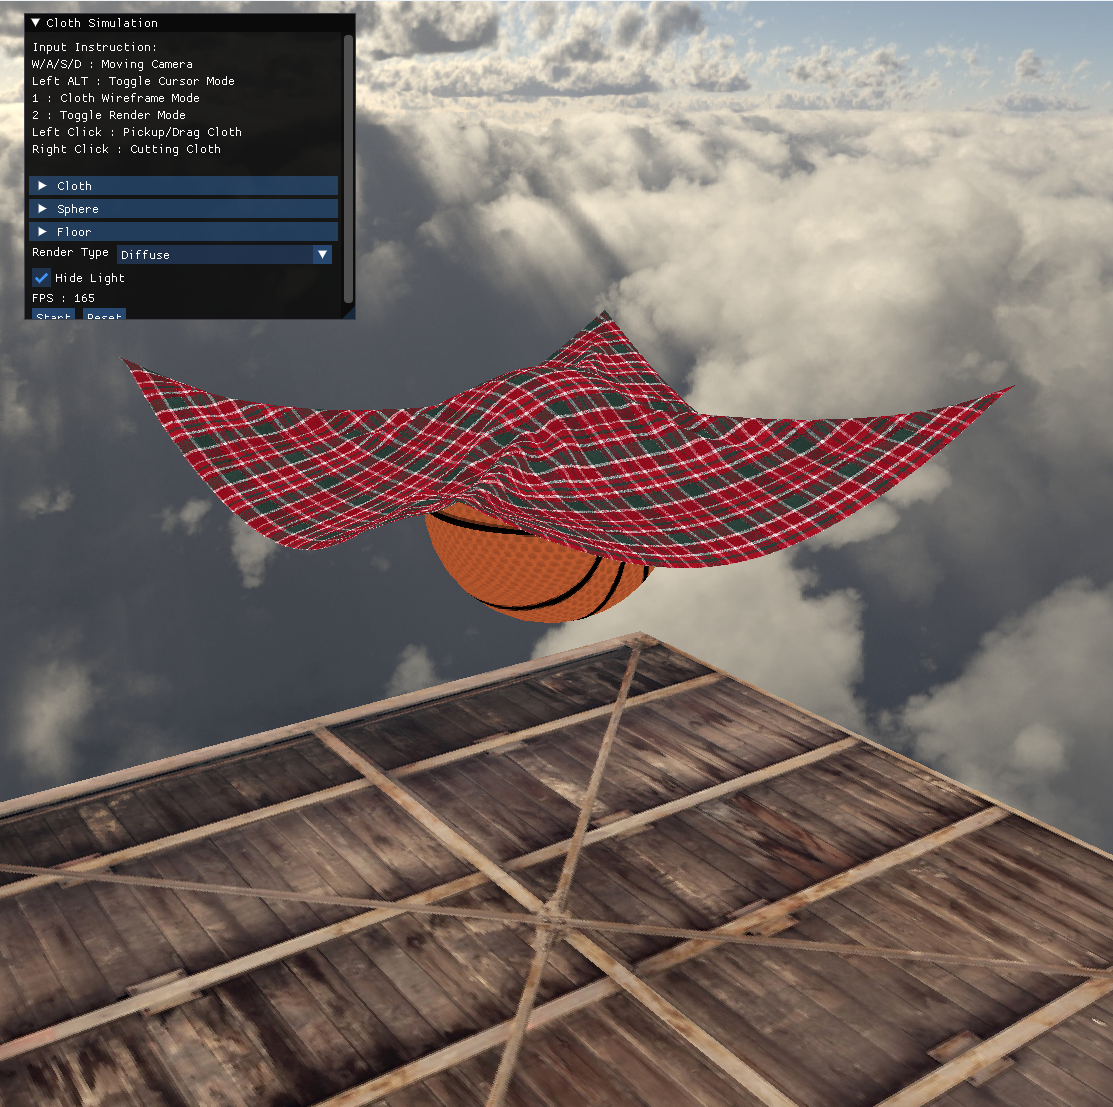
\includegraphics[scale = 0.2]{Deferred_Albedo}
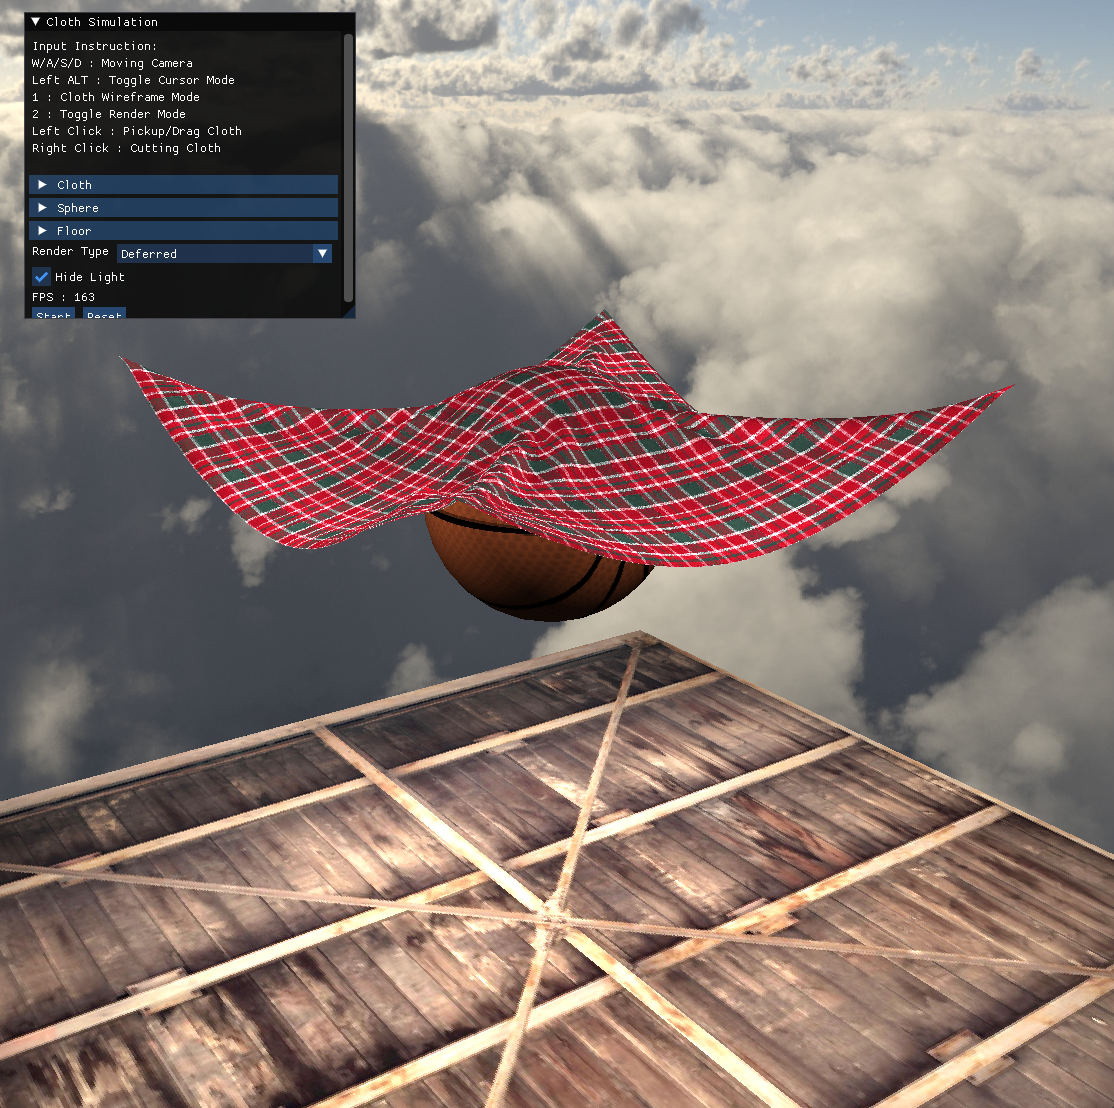
\includegraphics[scale = 0.2]{Deferred_Result}
[Figure 2.2.1.1 : Deferred Shading \\(Position + Normal + Albedo = Result)]\newline

\justifying
Overall, applying deferred shading technique will enhance the overall look of the simulation. Without lights and shadows, it will be harder to integrate the result of the physics computation.

\subsubsection{Cloth Interaction}
Compared to previous methods that we have implemented, The cloth interaction including dragging and cutting was the hardest part since there are a lot of variants we have to concern. Firstly, Dragging the cloth using a cursor is not as simple as we think because the screen is represented in 2D but our screen is 3D. We have to start with ray casting which will cast the ray from the camera to the scene for detecting that the ray is hitting any objects.
In this scenarios, we illustrate the mass spring point a box as well as let each points have their own collision bound.\newline

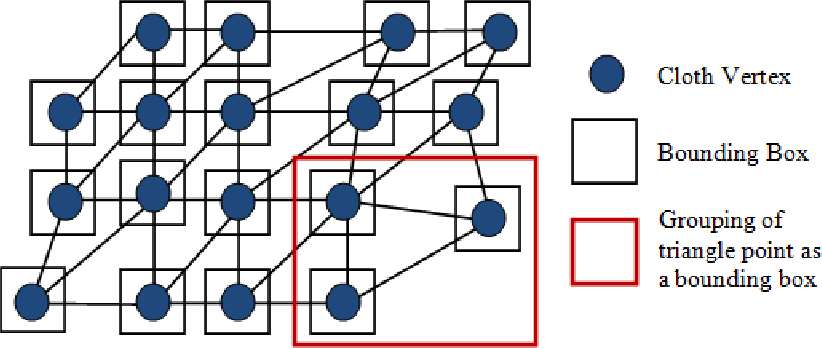
\includegraphics[width=\linewidth]{PointAABB}
\centering [Figure 2.2.2.1 : Bounding Box of Cloth Vertices]\newline

\justifying
After we create the bounding box of cloth's vertices, we have to convert the cursor position from Normalized Device Coordinate (NDCs) to Viewport Coordinate and then finalize it by converting from Viewport to World Coordinate. Since when we click the mouse, the clicked cursor will act as a ray and we can perform a ray casting by checking the collision between
ray and bounding box as known as (Ray vs AABB).\newline

\centering
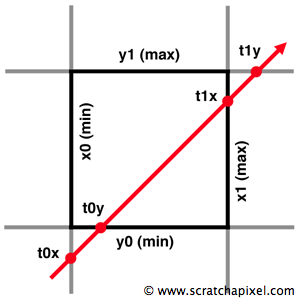
\includegraphics[scale = 0.4]{RayAABB}\newline
[Figure 2.2.2.2 : Intersection bewteen Ray and AABB]\newline

\justifying
After we complete the ray casting process, We can simply get the dragging point by casting the ray into the bounding box to query which mass spring points that the ray hit. Then, we can mouse that current point along the cursor.\\
\indent To cut the cloth, we can simplify the process by hiding the hit point as well as not using that point for calculating the force and rendering since hiding the point is much easier than deleting that point and handling the rest. Luckily, dragging and cutting does not need any additional compute because of the Hooke's Law which already handle that parts.\newline

\centering
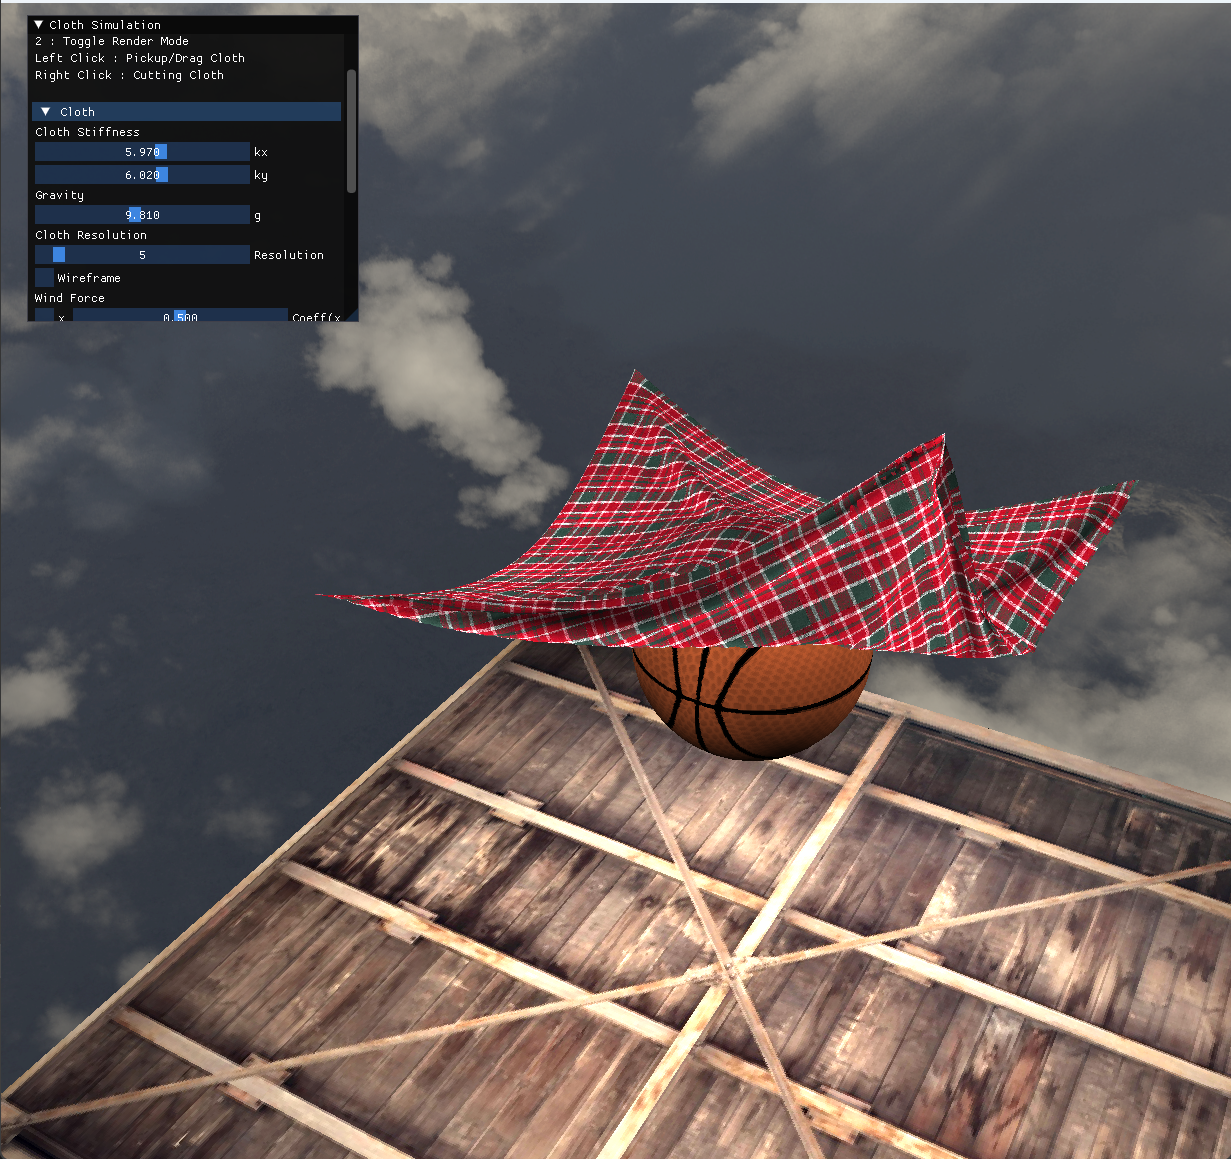
\includegraphics[scale = 0.15]{ClothDragging}
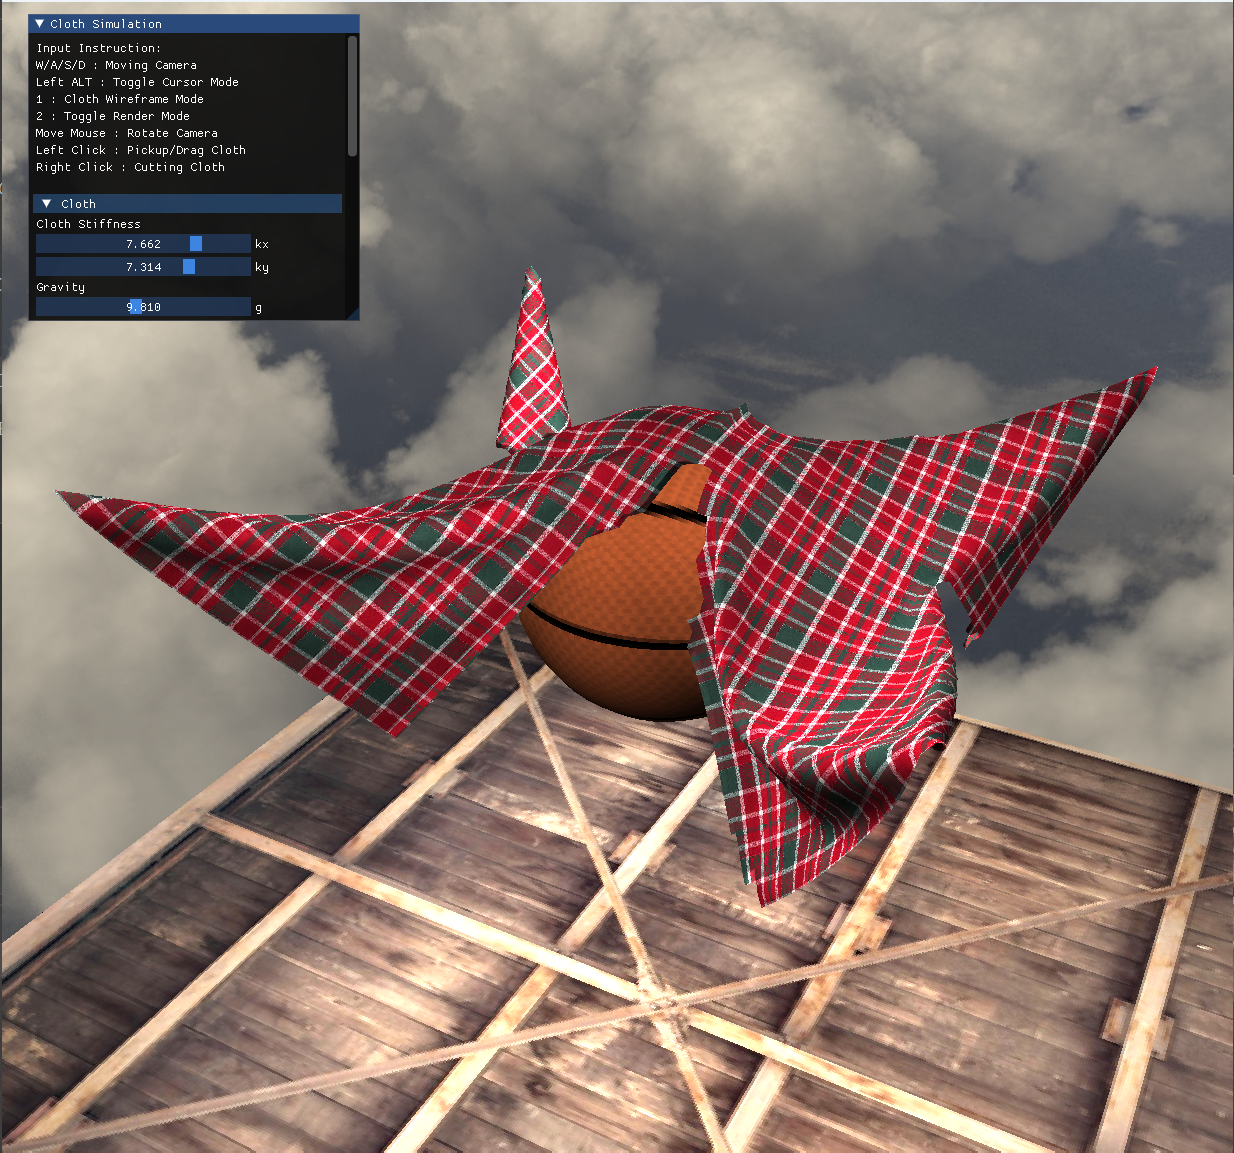
\includegraphics[scale = 0.15]{ClothCutting}\newline
[Figure 2.2.2.3 : Cloth Dragging \& Cutting]\newline

\justify
\section{Collision Handling}
to handle collision, the project will mainly focus on primitive including plane and sphere. The plane collision check is the simplest one since we can check the position on Y-Axis only. Alternatively, checking the collision with sphere need addition computation
which are calculating the length between the point and the center of the sphere. It will collide if the length between the point and sphere is greater than the sphere's radius itself.\newline

\raggedright
Sphere Collision:\\ 
\centering
$(c_x - p_x)^2 + (c_y - p_y)^2 + (c_z - p_z)^2  \leq  r^2$\newline

\raggedright
Note:\\
$c_x, c_y, c_z$ = Center position of sphere\\
$p_x, p_y, p_z$ = Position of cloth's mass spring point\newline 

\centering
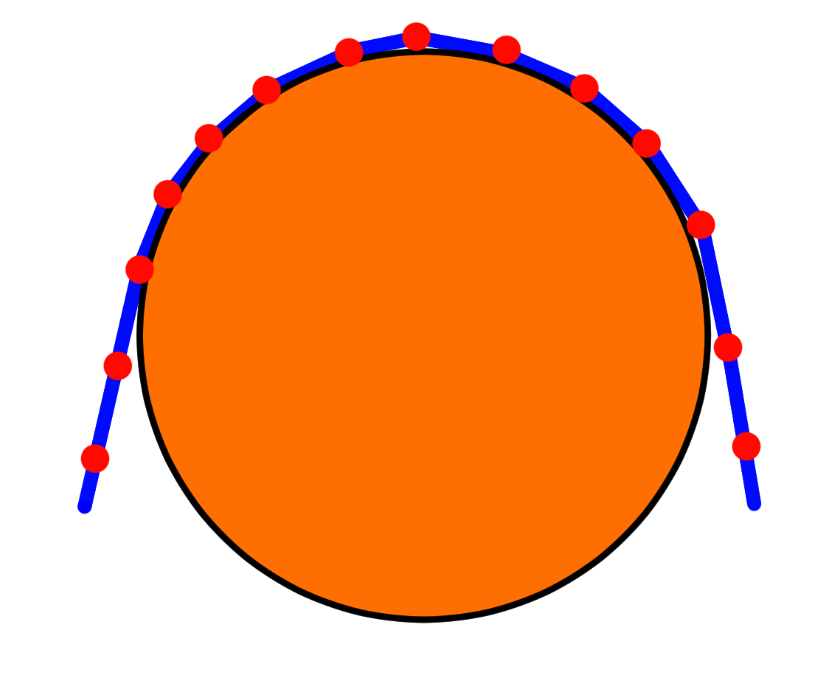
\includegraphics[scale = 0.25]{PointSphere}\newline
[Figure 3.1 : Point vs Sphere Collision]\newline

\raggedright
Floor Collision:\\
\centering
$p_y  \leq  f_y$\newline

\raggedright
Note:\\
$f_y$ = Position of floor (Y-Axis)\\
$p_y$ = Position of cloth's mass spring point (Y-Axis)\newline 

\section{Optimization}
\justify
In Optimization part, we will focus on how we can optimize the ray casting for cloth dragging and cutting. Bounding Volume Hierarchy are the one that was included in this project since it can decrease the number of query of ray casting by using the divide and conquer algorithm. 
Instead of computing using naive solution which cost $O(n)$, Bounding Volume Hierarchy consume lots of memory but it fasten the algorithm into $O(log\ n)$

\centering
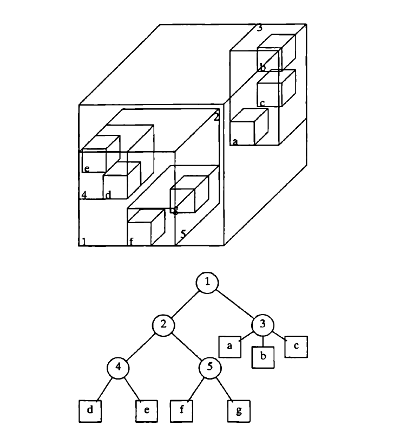
\includegraphics[width=\linewidth]{BVH}
[Figure 4.1 : Bounding Volume Hierarchy of Boxes]

\end{multicols}

\newpage
\section*{Reference}
\justify
Project Resource: \url{https://github.com/Siravich-NeeTer/PointMassSpring_Cloth}\newline\newline
[Figure 2.1.1] :\\ \url{https://ics.uci.edu/~shz/courses/cs114/docs/proj3/index.html}\newline
[Figure 2.2.2.1] :\\ \url{https://www.semanticscholar.org/paper/Collision-Detection-between-Cloth-and-a-Solid-using-Shapri-Sulaiman/2d800ea7059a2fe676060befcccd88461c05c618}\newline
[Figure 2.2.2.2] :\\ \url{https://www.scratchapixel.com/lessons/3d-basic-rendering/minimal-ray-tracer-rendering-simple-shapes/ray-box-intersection.html}\newline
[Figure 3.1] :\\ \url{https://docs.google.com/presentation/d/1y6XNUuwzDu5UHsI_M4QYHji3fY7xmwpD6t4UrOP7_Lo/edit?usp=sharing}\newline
[Figure 4.1] :\\ \url{https://computergraphics.stackexchange.com/questions/7828/difference-between-bvh-and-octree-k-d-trees}\newline\newline
Mass Spring Model:\\
\url{https://graphics.stanford.edu/courses/cs468-02-winter/Papers/Rigidcloth.pdf}\newline
\url{https://graphics.stanford.edu/~mdfisher/cloth.html}\newline
\url{https://andrewdcampbell.github.io/clothsim/}\newline\newline
Bounding Volume Hierarchy(BVH):\\
\url{https://github.com/madmann91/bvh}\newline\newline
RayCasting:\\
\url{https://antongerdelan.net/opengl/raycasting.html}\newline

\end{document}